\section{Beispiele zur Entwicklungsumgebung}
Hier zwei Beispiele zur Entwicklungsumgebung, welche Plattformunabhängig sind:
\begin{itemize}
\item 
In \vref{img:auctex} sehen wir ein Beispiel zur Entwicklungsumgebung \href{https://de.wikipedia.org/wiki/AUCTeX}{AUCTeX}.
\begin{figure}
	\centering
	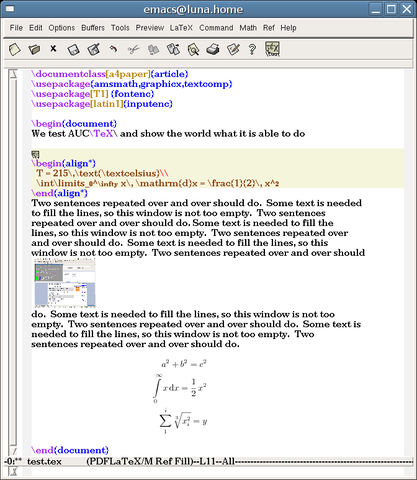
\includegraphics[width=.5\textwidth]{Auctex}
	\caption[Beispiel zur Entwicklungsumgebung AucTeX.]{AUCTeX ist eine Entwicklungsumgebung, die auf Emacs basiert. Hier ist Sie mit previewLaTeX im Einsatz}
	\label{img:auctex}
\end{figure}
\item
In \vref{img:eclipse} sehen wir ein Beispiel zur Entwicklungsumgebung \href{https://de.wikipedia.org/wiki/Eclipse_(IDE)}{Elcipse (IDE)}.
\begin{figure}
	\centering
	\pgfimage[width=.5\textwidth]{Eclipse}
	\caption[Eclipse (IDE) mit der Erweiterung TeXlipse.]{Ein virtuelles Beispiel für die Entwicklungsumgebung Eclipse (IDE) mit der Erweitung TeXlipse.}
	\label{img:eclipse}
\end{figure}
\end{itemize}


